% Compact replacement for utility_icra.tex; compile from the manuscript root.
\begingroup
\definecolor{teaserpale}{HTML}{303438}
\begin{tikzpicture}[x=1cm,y=.85cm,font=\sffamily\footnotesize,text=ink,>=Stealth]
\path[use as bounding box] (0,0) rectangle (17.8,4.4);
% Light image wells preserve the original opaque renders and their white pads.
\foreach \x/\w in {0/5.2,5.45/8.9,14.6/3.2}{\fill[white] (\x,1.21) rectangle ++(\w,2.47);}
\foreach \x/\w in {0/5.2,5.45/8.9,14.6/3.2}{
 \fill[teaserpale] (\x,3.84) rectangle ++(\w,.5);
 \draw[steel,line width=1pt] (\x,4.34)--++(\w,0);
}
\node[anchor=west,font=\sffamily\bfseries\footnotesize] at (.12,4.09) {(a) Grasp Prediction};
\node[anchor=west,font=\sffamily\bfseries\footnotesize] at (5.57,4.09) {(b) Contact-Based Retargeting};
\node[anchor=west,font=\sffamily\bfseries\footnotesize] at (14.72,4.09) {(c) Refinement};
\node[inner sep=0pt] at (1.35,2.43) {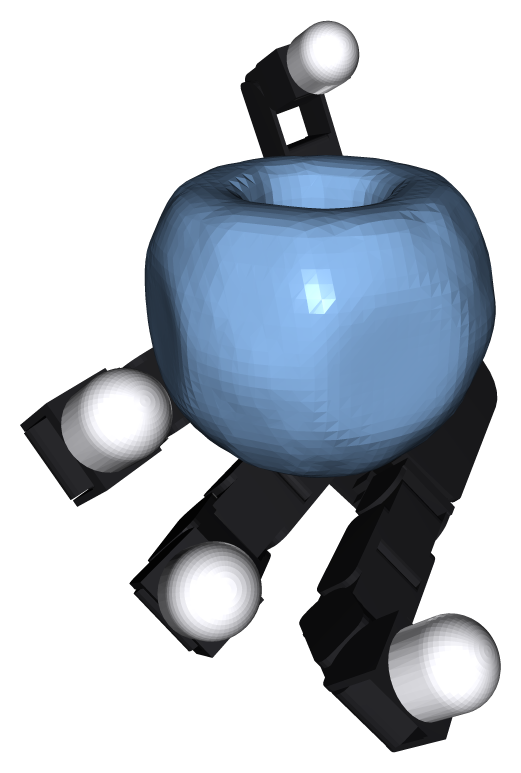
\includegraphics[height=2.05cm,width=2.45cm,keepaspectratio]{figures/generated_raw.png}};
\node[inner sep=0pt] at (3.92,2.43) {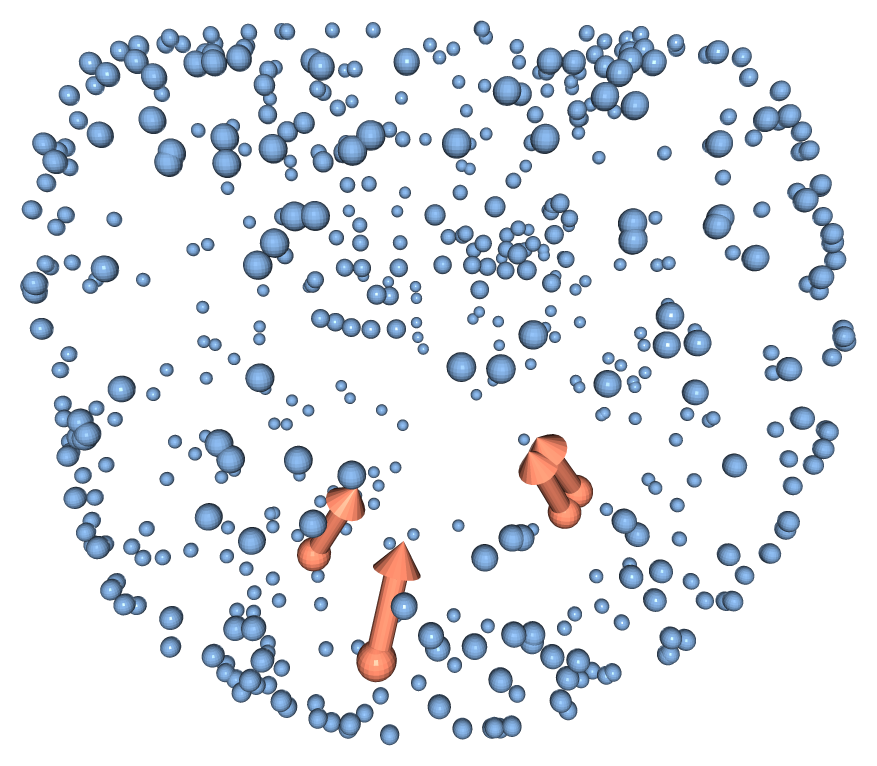
\includegraphics[height=2.05cm,width=2.45cm,keepaspectratio]{figures/generated_predictions.png}};
\node at (1.35,1.01) {Wrist $T$, joints $q$};
\node at (3.92,1.01) {Contacts $C$, forces $F$};
\node[inner sep=0pt] at (6.67,2.43) {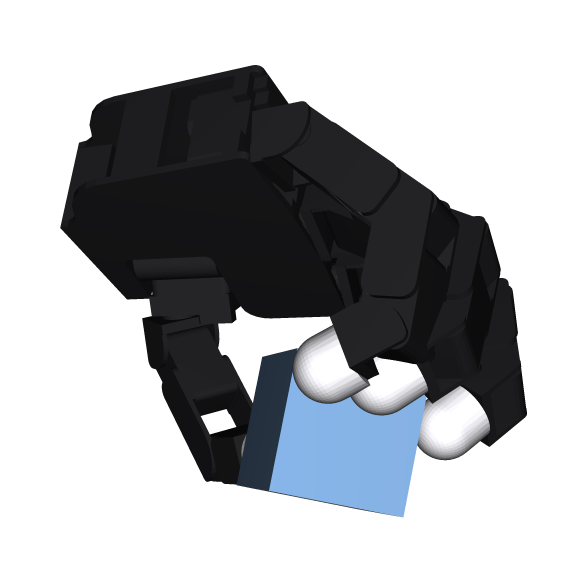
\includegraphics[height=2.05cm,width=2.2cm,keepaspectratio]{figures/teaser_source/selected_allegro.png}};
\node[inner sep=0pt] at (9.56,2.43) {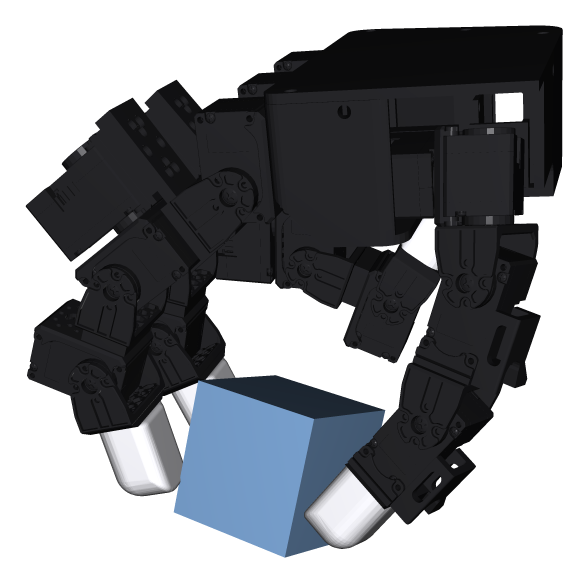
\includegraphics[height=2.05cm,width=2.2cm,keepaspectratio]{figures/teaser_source/selected_leap.png}};
\node[inner sep=0pt] at (12.82,2.43) {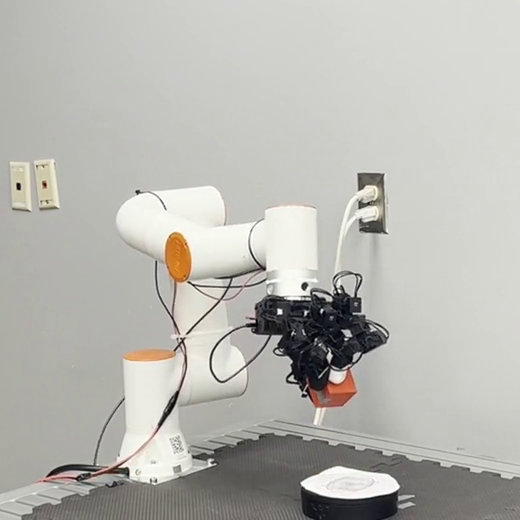
\includegraphics[height=2.05cm,width=2.3cm,keepaspectratio,trim=185bp 70bp 80bp 195bp,clip]{figures/webpage_phases/cube_0_lift.png}};
\draw[->,coral,line width=1pt] (7.85,2.43)--(8.36,2.43);
\node[font=\sffamily\scriptsize,align=center,text=black] at (8.10,3.25) {Retarget\\+ refine};
\draw[->,coral,line width=1pt] (10.76,2.43)--(11.47,2.43);
\node[font=\sffamily\scriptsize,align=center,text=black] at (11.11,3.25) {Robot\\execution};
\node at (6.67,1.01) {Allegro};
\node at (9.56,1.01) {LEAP};
\node at (12.82,1.01) {Hardware example};
\node[inner sep=0pt] at (16.2,2.43) {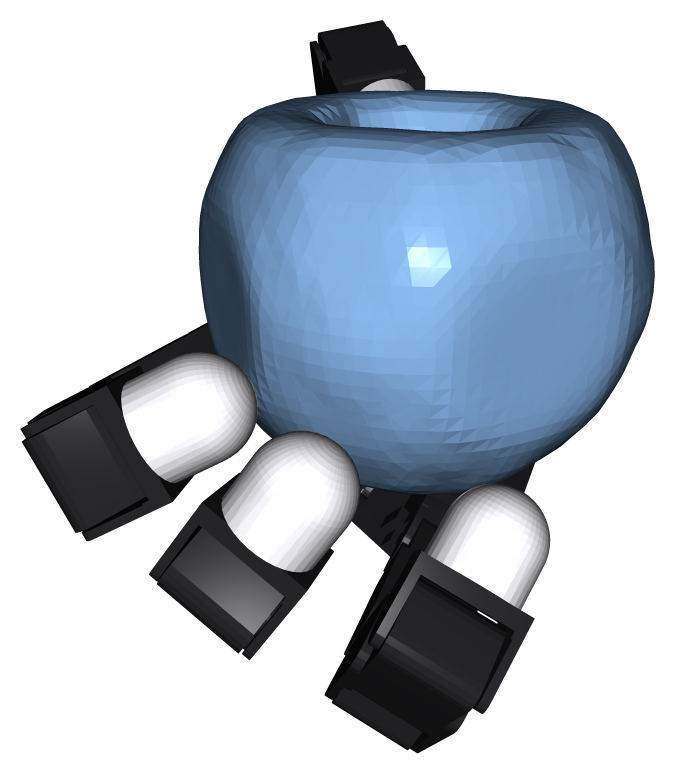
\includegraphics[height=2.05cm,width=2.9cm,keepaspectratio]{figures/generated_refined.png}};
\node at (16.2,1.01) {Surface fit of (a)};
% Scope is wrist-flow equivariance, not equivariance of every decoded quantity.
\fill[teaserpale] (0,.03) rectangle (17.8,.67);
\node[anchor=west,font=\sffamily\bfseries\footnotesize] at (.13,.35) {Wrist-Flow Equivariance};
\node at (7.0,.35) {$T(gP;gT_0)=g\,T(P;T_0)$};
\node[anchor=east,font=\sffamily\scriptsize] at (17.65,.35) {8 comparisons: $\Delta R<6.1\!\times\!10^{-6}$ deg; $\Delta t<1.2\!\times\!10^{-7}$ m};
\end{tikzpicture}
\endgroup
